\documentclass[11pt,english]{beamer}
%\documentclass[11pt]{beamer}
\usepackage{mathptmx}
\renewcommand{\sfdefault}{lmss}
\renewcommand{\familydefault}{\sfdefault}
\usepackage[T1]{fontenc}
\usepackage[latin9]{inputenc}
\usepackage{amsmath}
\usepackage{amssymb}
\usepackage{graphicx}
\PassOptionsToPackage{normalem}{ulem}
\usepackage{ulem}
\usepackage{caption}
\captionsetup{labelformat=empty}
\usepackage{bbm}
\usepackage{upgreek}
\usepackage{graphicx}
\setbeamertemplate{section in toc}[sections numbered]
\makeatletter
\usepackage{caption} 
\captionsetup[table]{skip=10pt}
%%%%%%%%%%%%%%%%%%%%%%%%%%%%%% Textclass specific LaTeX commands.
 % this default might be overridden by plain title style
 \newcommand\makebeamertitle{\frame{\maketitle}}%
 % (ERT) argument for the TOC
 \AtBeginDocument{%
   \let\origtableofcontents=\tableofcontents
   \def\tableofcontents{\@ifnextchar[{\origtableofcontents}{\gobbletableofcontents}}
   \def\gobbletableofcontents#1{\origtableofcontents}
 }


\setbeamersize{text margin left= .8em,text margin right=1em} 
\newenvironment{wideitemize}{\itemize\addtolength{\itemsep}{10pt}}{\enditemize}
\newenvironment{wideitemizeshort}{\itemize}{\enditemize}

%%%%%%%%%%%%%%%%%%%%%%%%%%%%%% User specified LaTeX commands.
%\documentclass[presentation]{beamer}


\def\Tiny{\fontsize{7pt}{8pt}\selectfont}
\def\Normal{\fontsize{8pt}{10pt}\selectfont}

\usetheme{Madrid}
\usecolortheme{lily}
%\setbeamercovered{transparent}
\useinnertheme{rounded}


\setbeamertemplate{footline}{\hfill\Normal{\insertframenumber/\inserttotalframenumber}}
%\setbeamertemplate{footline}{}

\setbeamertemplate{navigation symbols}{}

\newenvironment{changemargin}[2]{%
\begin{list}{}{%
\setlength{\topsep}{0pt}%
\setlength{\leftmargin}{#1}%
\setlength{\rightmargin}{#2}%
\setlength{\listparindent}{\parindent}%
\setlength{\itemindent}{\parindent}%
\setlength{\parsep}{\parskip}% 
}%
\item[]}{\end{list}}

\setbeamertemplate{footline}{\hfill\insertframenumber/\inserttotalframenumber}
\setbeamertemplate{navigation symbols}{}

%\usepackage{times}  % fonts are up to you
\usepackage{graphicx}
%\usepackage{graphics}
\usepackage{epsfig}
\usepackage{bm}
\usepackage{epsf}
\usepackage{float}
\usepackage[final]{pdfpages}
\usepackage{multirow}
\usepackage{colortbl}
\usepackage{xkeyval}
%\usepackage{sgame}
%\usepackage{pst-node}
\usepackage{listings}
\usepackage{ifthen}
%\usepackage{hyperref}
\usepackage{tikz}

%\usepackage{times}  % fonts are up to you
%\usepackage{graphicx}
%\usepackage{graphics}
\usepackage{epsfig,bm,epsf,float}
\usepackage[final]{pdfpages}
\usepackage{xcolor,multirow,colortbl}
\usepackage{xkeyval}
\usepackage{verbatim}
%\usepackage{sgame}
%\usepackage{pst-node}
\usepackage{listings}
%\usepackage{handoutWithNotes}
%\pgfpagesuselayout{3 on 1 with notes}[letterpaper,border shrink=5mm]
%\pgfpagesuselayout{2 on 1 with notes landscape}[letterpaper,border shrink=5mm]
\usepackage{setspace}
\usepackage{ragged2e}

\setbeamersize{text margin left=1em,text margin right=1em} % CambridgeUS spacing if you use default instead


%\pdfmapfile{+sansmathaccent.map}

% Table formatting
\usepackage{booktabs}


% Decimal align
\usepackage{dcolumn}
\newcolumntype{d}[0]{D{.}{.}{5}}

\newcommand\independent{\protect\mathpalette{\protect\independenT}{\perp}}
\def\independenT#1#2{\mathrel{\rlap{$#1#2$}\mkern2mu{#1#2}}}

\global\long\def\expec#1{\mathbb{E}\left[#1\right]}
\global\long\def\var#1{\mathrm{Var}\left[#1\right]}
\global\long\def\cov#1{\mathrm{Cov}\left[#1\right]}
\global\long\def\prob#1{\mathrm{Prob}\left[#1\right]}
\global\long\def\one{\mathbf{1}}
\global\long\def\diag{\operatorname{diag}}
\global\long\def\expe#1#2{\mathbb{E}_{#1}\left[#2\right]}
\DeclareMathOperator*{\plim}{\text{plim}}

%\usefonttheme[onlymath]{serif}

\usepackage{appendixnumberbeamer}
\renewcommand{\thefootnote}{}

\setbeamertemplate{footline}
        {
      \leavevmode%
   %   \hbox{%
%      \begin{beamercolorbox}[wd=\paperwidth,ht=2.25ex,dp=1ex,right]{date in head/foot}%
        %\usebeamerfont{date in head/foot}\insertshortdate{}\hspace*{2em}%
\hfill
    %turning the next line into a comment, erases the frame numbers
        \insertframenumber{}\hspace*{2ex}\vspace{1ex}

  %    \end{beamercolorbox}}%
}

\definecolor{blue}{RGB}{0, 0, 210}
\definecolor{red}{RGB}{170, 0, 0}

\makeatother

\usepackage[english]{babel}

%\mode<handout>{
  %\setbeamercolor{background canvas}{bg=black!5}
  %\usepackage{pgfpages}
  %\pgfpagesuselayout{2 on 1}[a4paper,border shrink=5mm]
 %\pgfpagesuselayout{4 on 1}[a4paper,border shrink=5mm,landscape]
%}
%\newcommand{\opause}{\pause{}} 

\usepackage{tikz}
\newcommand*\circled[1]{\tikz[baseline=(char.base)]{             \node[circle,ball color=structure.fg, shade,   color=white,inner sep=1.2pt] (char) {\tiny #1};}} 

\makeatletter
\let\save@measuring@true\measuring@true
\def\measuring@true{%
  \save@measuring@true
  \def\beamer@sortzero##1{\beamer@ifnextcharospec{\beamer@sortzeroread{##1}}{}}%
  \def\beamer@sortzeroread##1<##2>{}%
  \def\beamer@finalnospec{}%
}
\makeatother

\begin{document}

%% Title slide
\begin{frame}[noframenumbering]{}
\vspace{0.5cm}
\title[]{Day 3: On Formulas and Models}
\author{Peter Hull}
\date{Design-Based Regression Inference \\Spring 2024} 
\titlepage {\small{}\ }\thispagestyle{empty} \vspace{-30pt}

\end{frame}
 

\begin{frame}{Outline}

1. Formula Treatments/Instruments
\vspace{0.8cm}

2. Structural Models

\end{frame}

\begin{frame}{Beyond Simple Treatments/Instruments}

\begin{itemize}
\item We've seen how a regression of $y_i$ on $x_i$ and $w_i$ identifies a convex average of treatment effects when $E[x_i\mid y_i(\cdot),w_i]=E[x_i\mid w_i]=w_i^\prime\gamma$\smallskip
\begin{itemize}
\item For IV: $E[z_i\mid y_i(\cdot),w_i]=w_i^\prime\gamma$ and exclusion/monotonicity hold
\end{itemize}\bigskip\pause{}
\item This gives us a strategy for robustly estimating causal effects with ``formula'' treatments/instruments, constructed from some exogenous shocks and other non-random variables\pause{}. E.g.: \smallskip
\begin{itemize}
\item Interacted treatments: $x_i=s_ig_i$, with exogenous shocks $g_i$\smallskip\pause{}
\item Shift-share instruments: $z_i=\sum_k s_{ik} g_k$, with exogenous shocks $\{g_k\}_{k=1}^K$\smallskip\pause{}
\item Spillover treatments: e.g. number of neighbors treated in an RCT\smallskip\pause{}
\item Instruments for policy eligibility, combining exogenous policy shocks \& non-random measures of policy exposure (e.g. income/family structure)
\end{itemize}\bigskip\pause{}
\item Let's build up to these slowly...
\end{itemize}

\end{frame}

\begin{frame}{Interacted Treatments}
\begin{itemize}
\item Suppose $g_i\mid y(\cdot),s\stackrel{iid}{\sim} G$ for some observed $s_i$ \smallskip
\begin{itemize}
\item E.g. $g_i$ drawn in a simple RCT, with $s_i$ being a baseline characteristics\smallskip\pause
\item We are interested in the effects of $x_i=s_ig_i$: e.g. heterogeneous effects \smallskip\pause{}
\item Perhaps estimated alongside direct effects of $g_i$ (but don't worry about multiple treatments for now)
\end{itemize}\bigskip\pause{}
\item The design-based approach says we need to adjust for:
\begin{align*}
E[x_i\mid s]=\pause{}E[s_i g_i\mid s]=\pause{}s_i E[g_i]=\pause{} s_i \mu
\end{align*}\pause{}
I.e. need to control for $s_i$ to just leverage the random variation in $g_i$\smallskip\pause{}
\begin{itemize}
\item Can use $s_ig_i$ as an IV controlling for $s_i$, given exclusion/monotonicity
\end{itemize}
\end{itemize}
\end{frame}

\begin{frame}{Interacted Treatments (Cont.)}
\begin{itemize}
\item Now suppose $g_i\mid y(\cdot),s,q\stackrel{iid}{\sim} G(q_i)$: e.g., a stratified RCT \smallskip
\begin{itemize}
\item Again, we want to estimate the effects of $x_i=s_ig_i$ (or use it as an IV)
\end{itemize}\bigskip\pause{}
\item Now, for $\mu(q_i)=E[g_i\mid q_i]$:
\begin{align*}
E[x_i\mid s,q]=E[s_i g_i\mid s,q]=s_i E[g_i\mid s,q]=s_i \mu(q_i)\pause{}
\end{align*}
I.e. need to control for $s_i$ interacted with a flexible function of $q_i$\smallskip
\begin{itemize}
\item E.g. the interactions of $s_i$ and strata fixed effects
\end{itemize}\bigskip\pause{}
\item Key point: the design of exogenous shocks $g_i$ + knowledge of the ``formula'' $s_i g_i$ tells us what controls are needed for identification
\end{itemize}
\end{frame}

\begin{frame}{Shift-Share Instruments}
\begin{itemize}
\item Now suppose the shocks $g_k\mid y(\cdot),s\stackrel{iid}{\sim} G$ vary at a different ``level'' $k$, and we want to estimate effects with $z_i=\sum_k s_{ik} g_k$\smallskip\pause{}
\begin{itemize}
\item E.g. $g_k$ are shocks to industries $k$ and $s_{ik}\in(0,1)$ are regional measures of shock exposure, perhaps with $\sum_k s_{ik}=1$ for all $i$
\end{itemize}\bigskip\pause{}
\item What is the ``expected instrument''?
\begin{align*}
E[z_i\mid s]=\pause{} E\left[\sum_k s_{ik} g_k\mid s\right]=\pause{}\sum_k s_{ik} E[g_k] =\pause{} \left(\sum_k s_{ik}\right)\mu
\end{align*}\pause{}
\begin{itemize}
\item I.e. need to control for the ``sum of shares'' $w_i=\sum_k s_{ik}$ (which may be one, in which case no controls needed!)
\end{itemize}\bigskip\pause{}
\item Cool new twist: we can use design to ``translate'' shocks from one level (e.g. industries) to estimate effects at another (e.g. regions)!
\end{itemize}
\end{frame}

\begin{frame}{Shift-Share Instruments (Cont.)}
\begin{itemize}
\item Now suppose $E[g_k\mid y(\cdot),s,q]=q_k^\prime \mu$, still with $z_i=\sum_k s_{ik} g_k$\smallskip\pause{}
\begin{itemize}
\item E.g. Autor et al. (2014) leverage industry shocks $g_k$ from China over two periods, with $q_k$ being a set of period FE\smallskip\pause{}
\item Want to only use within-period shock variation: e.g. shocks and unobservables could have different means across time
\end{itemize}\bigskip\pause{}
\item What is the ``expected instrument''?
\begin{align*}
E[z_i\mid s,q]= E\left[\sum_k s_{ik} g_k\mid s,q\right]=\sum_k s_{ik} E[g_k\mid q_k] =\left(\sum_k s_{ik}q_k\right)^\prime\mu
\end{align*}\pause{}
\begin{itemize}
\item I.e. need to control for the share-weighted average of shock-level confounders, $w_i=\sum_k s_{ik}q_k$\smallskip\pause{}
\item In Autor et al. (2014), this means controlling for the sum-of-shares interacted with period FE
\end{itemize}
\end{itemize}
\end{frame}

\begin{frame}{Example: Autor et al. (2014)}

\begin{center}
	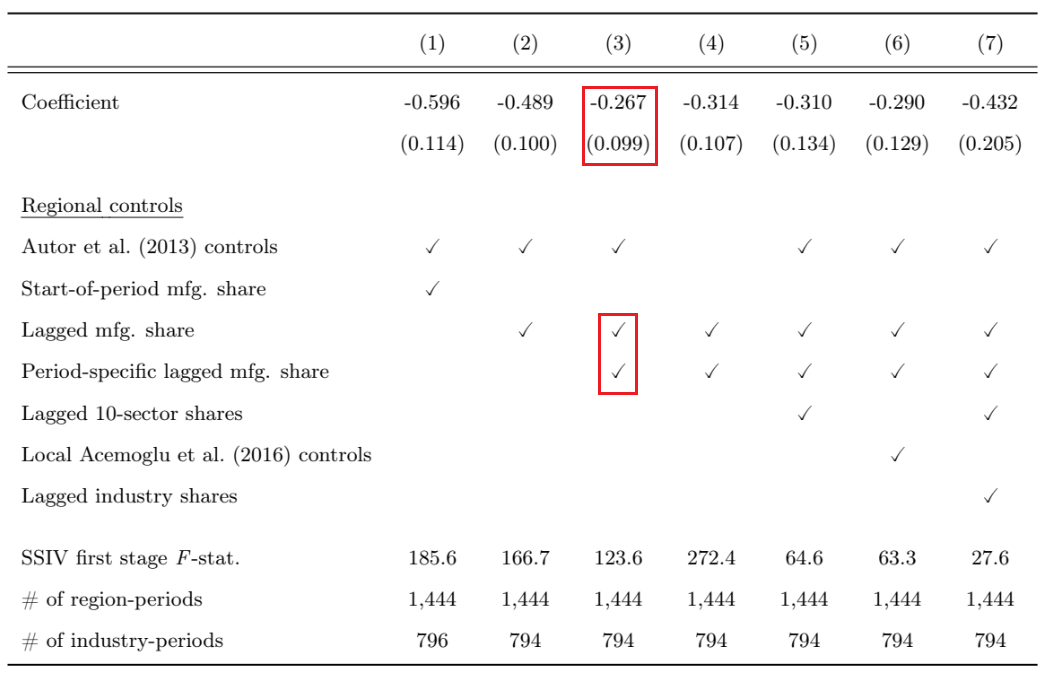
\includegraphics[width=0.9\textwidth]{figures/adh_bhj.png}
\end{center}

From Borusyak et al. (2022); check out my SSIV mixtape for more!


\end{frame}

\begin{frame}{Formula Instruments: General Case}
\begin{itemize}
\item We have a $z_i=f_i(g,s)$ for known $f_i(\cdot)$ and observed $g$ and $s$\smallskip
\begin{itemize}
\item We assume $g\mid y(\cdot),w\sim G(w)$ for $w=(s,q)$ and known $G(\cdot)$\smallskip\pause{}
\item E.g. $G(\cdot)$ is given by a randomization protocol or specifies permutations of the shocks which are as-good-as-random\smallskip\pause{}
\item Shocks may vary at a different ``level'' than observations
\end{itemize}\bigskip\pause{}
\item Design-based approach: include controls that span $\mu_i=E[f_i(g,s)\mid w]$\smallskip\pause{}
\begin{itemize}
\item Or use ``recentered'' instrument $\tilde{z}_i=z_i-\mu_i$ (same estimand)
\end{itemize}\bigskip\pause{}
\item For complex designs, $\mu_i$ can be computed by simulation:\smallskip
\begin{enumerate}
\item Redraw counterfactual shocks $g^{(\ell)}$ from $G(w)$, $\ell=1,\dots,L$ \smallskip\pause{}
\item Recompute the IV w/these shocks, holding else fixed: $z_i^{(\ell)}=f_i(g^{(\ell)},s)$\smallskip\pause{}
\item Compute expected instrument as $\mu_i=\frac{1}{L}\sum_\ell z_i^{(\ell)}$
\end{enumerate}
\end{itemize}
\end{frame}

\begin{frame}{Example: Borusyak and Hull (2023)}
\begin{itemize}
\item BH are interested in estimating the effect of market access on employment by leveraging changes in the transportation network\smallskip
\begin{itemize}
\item Market access specifies (using economic theory) how transportation upgrades affect economic integration across a country (i.e. spillovers)\smallskip\pause{}
\item Upgrades (of e.g. rail lines) at a different level than regional outcomes
\end{itemize}\bigskip\pause{}
\item They use the differential timing of high-speed rail (HSR) construction in China, conditional on construction plans, as exogenous shocks\smallskip\pause{}
\begin{itemize}
\item Basic idea: permute which planned lines opened by some date conditional on line observables to generate counterfactual shocks\smallskip\pause{}
\item Then either control for or recenter by expected market access growth
\end{itemize}
\end{itemize}
\end{frame}

\begin{frame}{HSR Lines and Market Access}

\begin{center}
	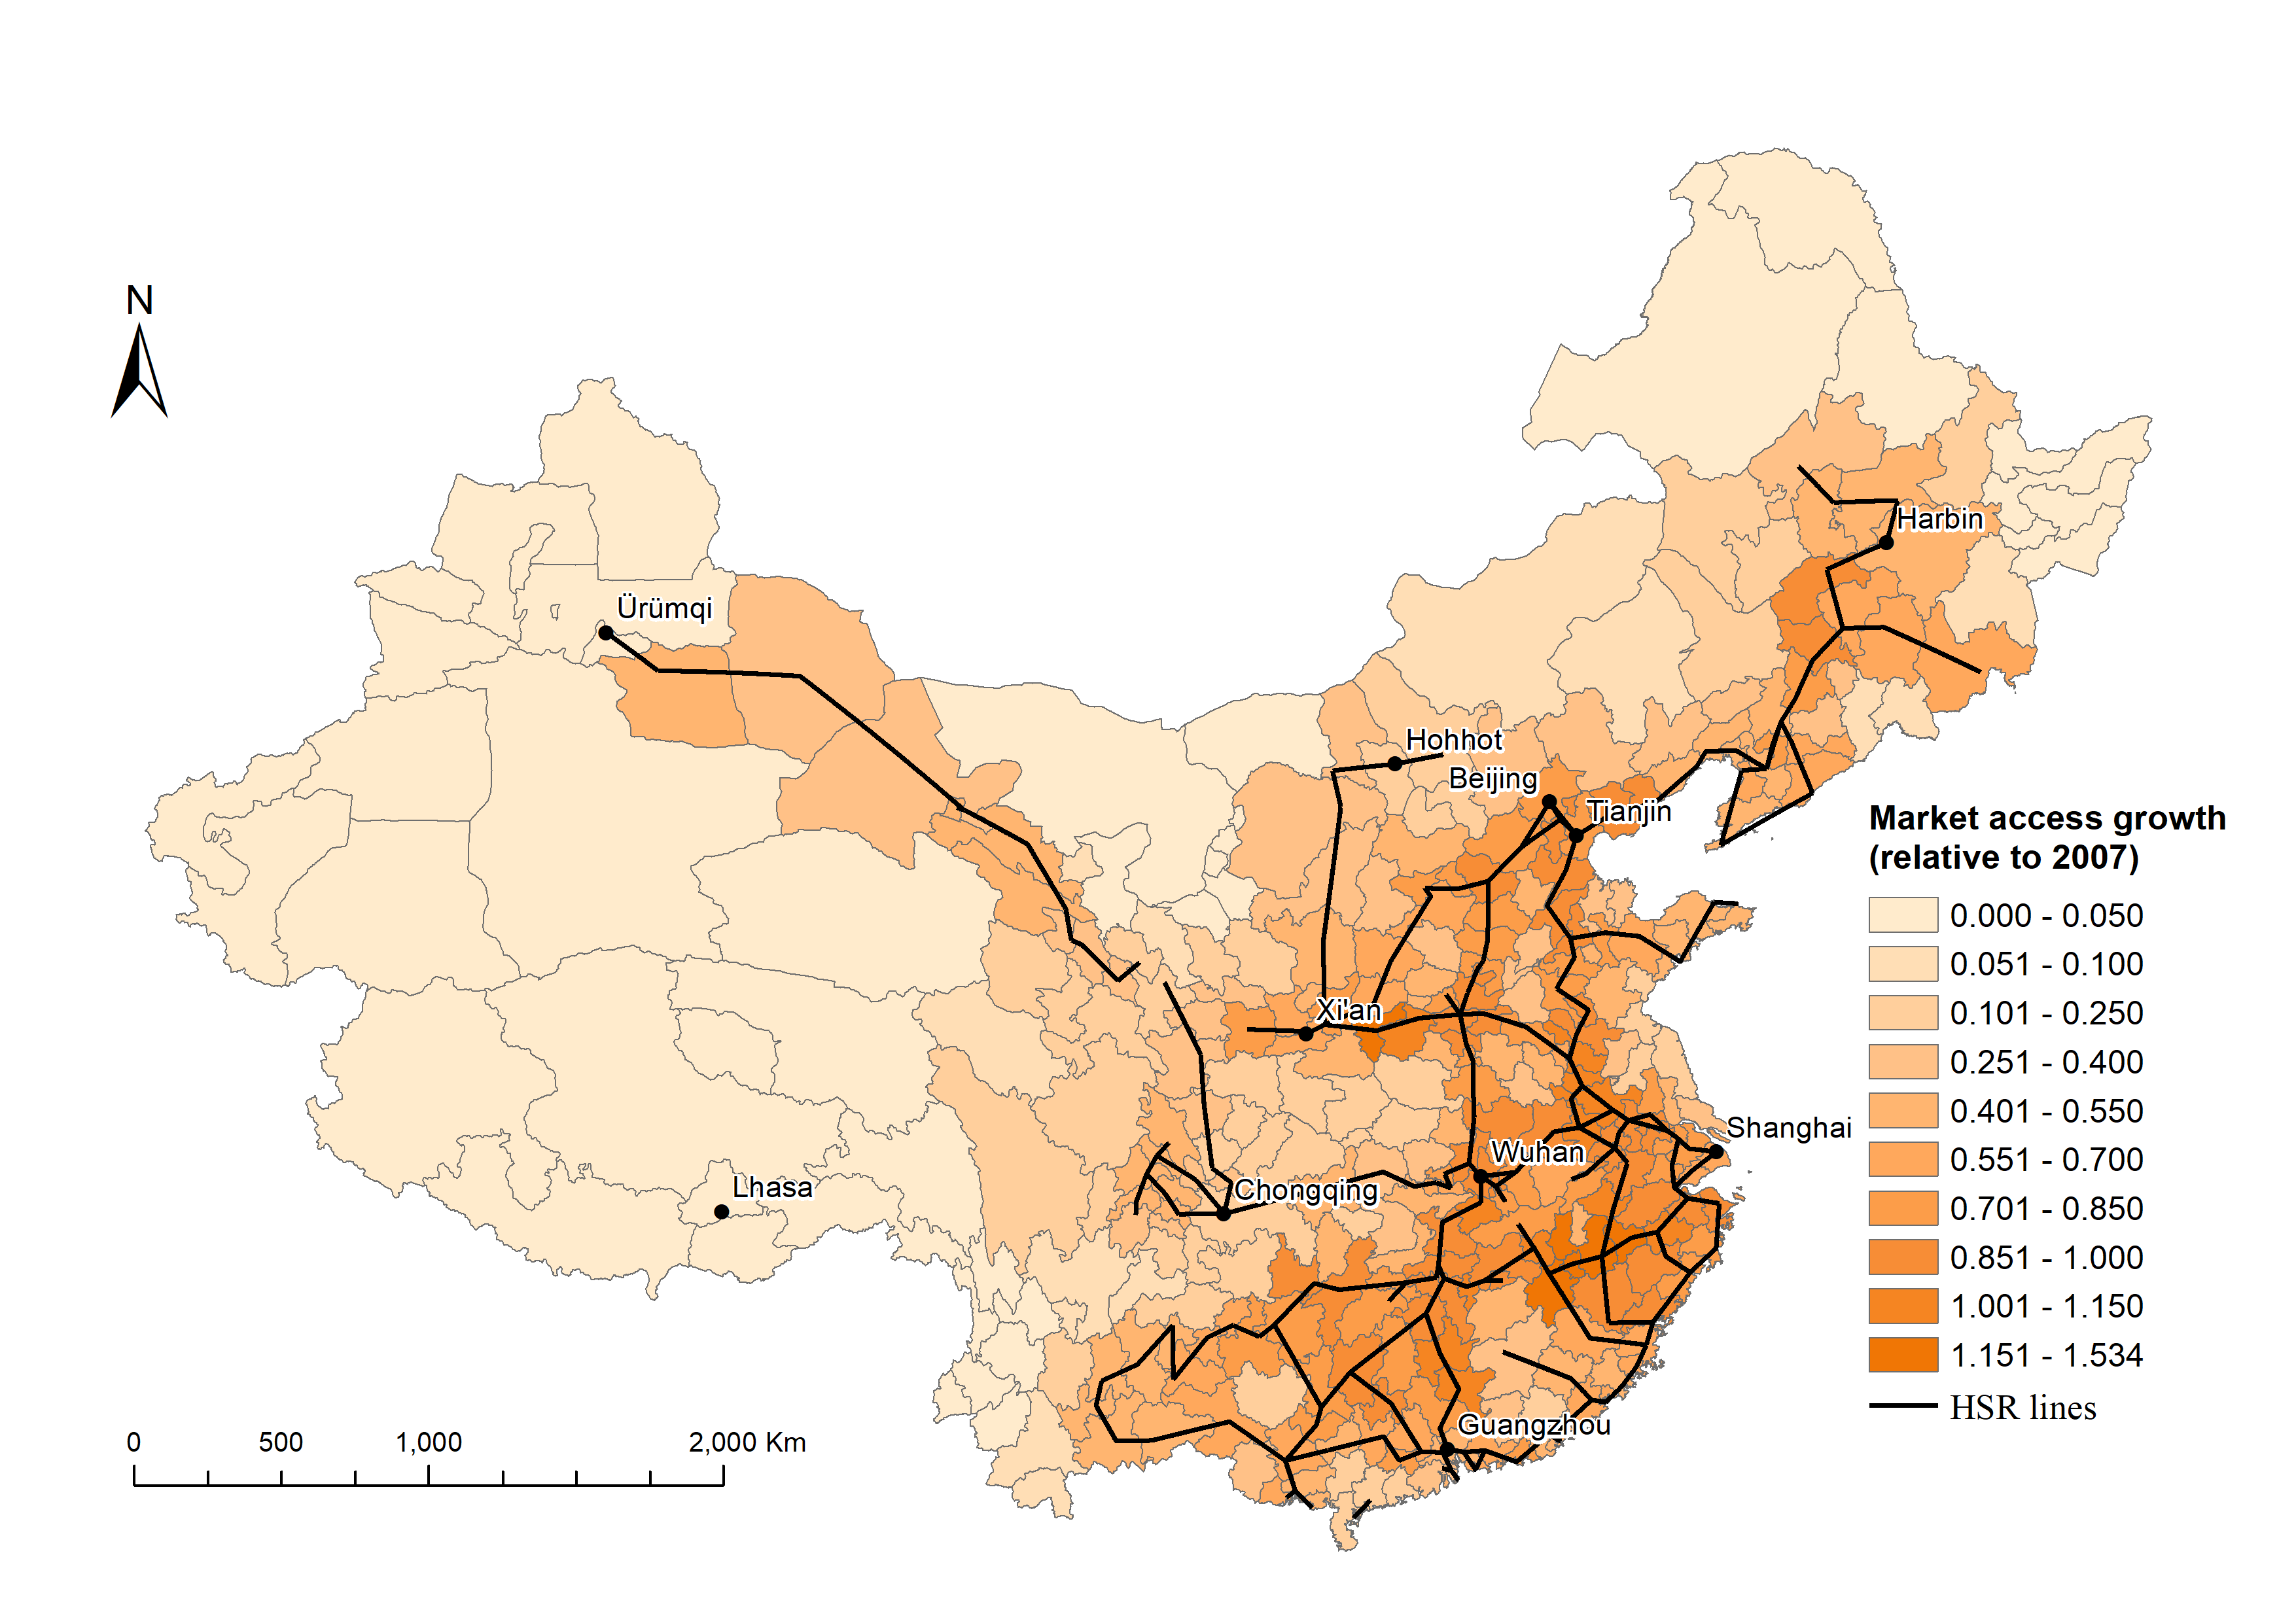
\includegraphics[width=0.9\textwidth]{figures/Line_panel2016.png}
\end{center}

Naive OLS compares dark (``treatment'') vs light (``control'') regions

\end{frame}

\begin{frame}{HSR Lines and Counterfactuals}

\begin{center}
	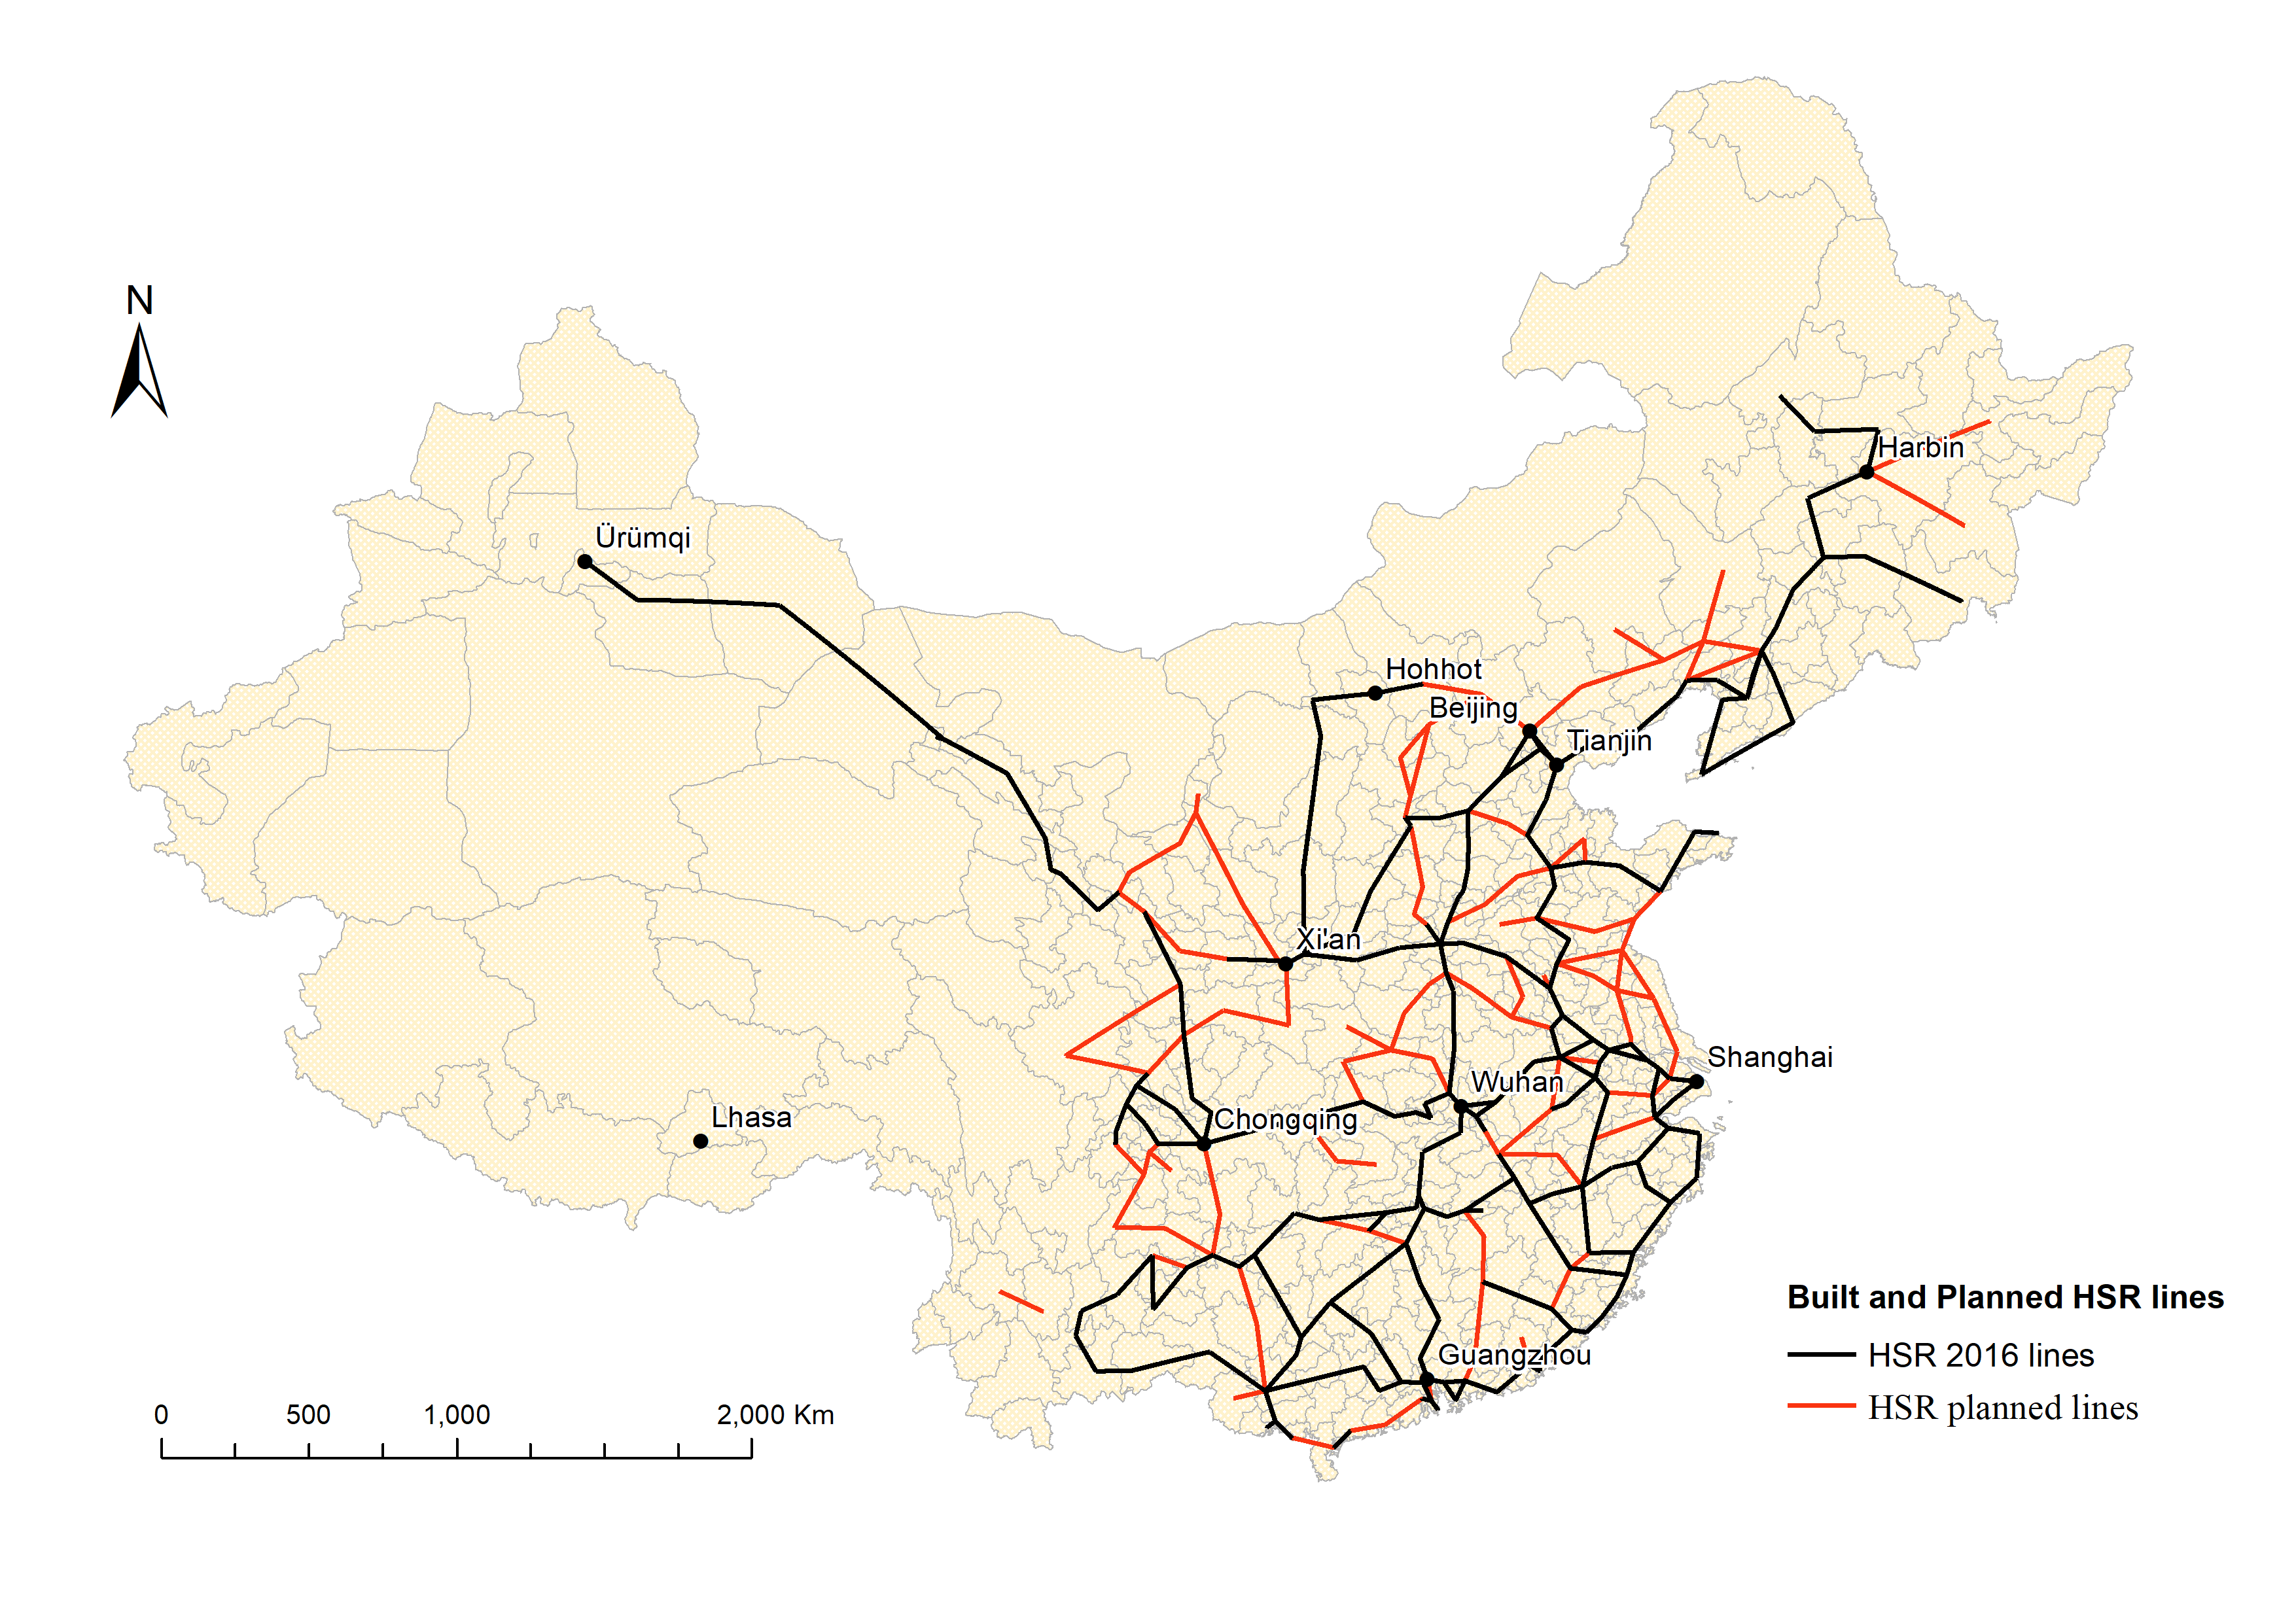
\includegraphics[width=0.9\textwidth]{figures/Lines_actual_planned.png}
\end{center}

Counterfactuals permute which lines opened by 2016, conditional on length

\end{frame}

\begin{frame}{BH Estimates}

\begin{center}
	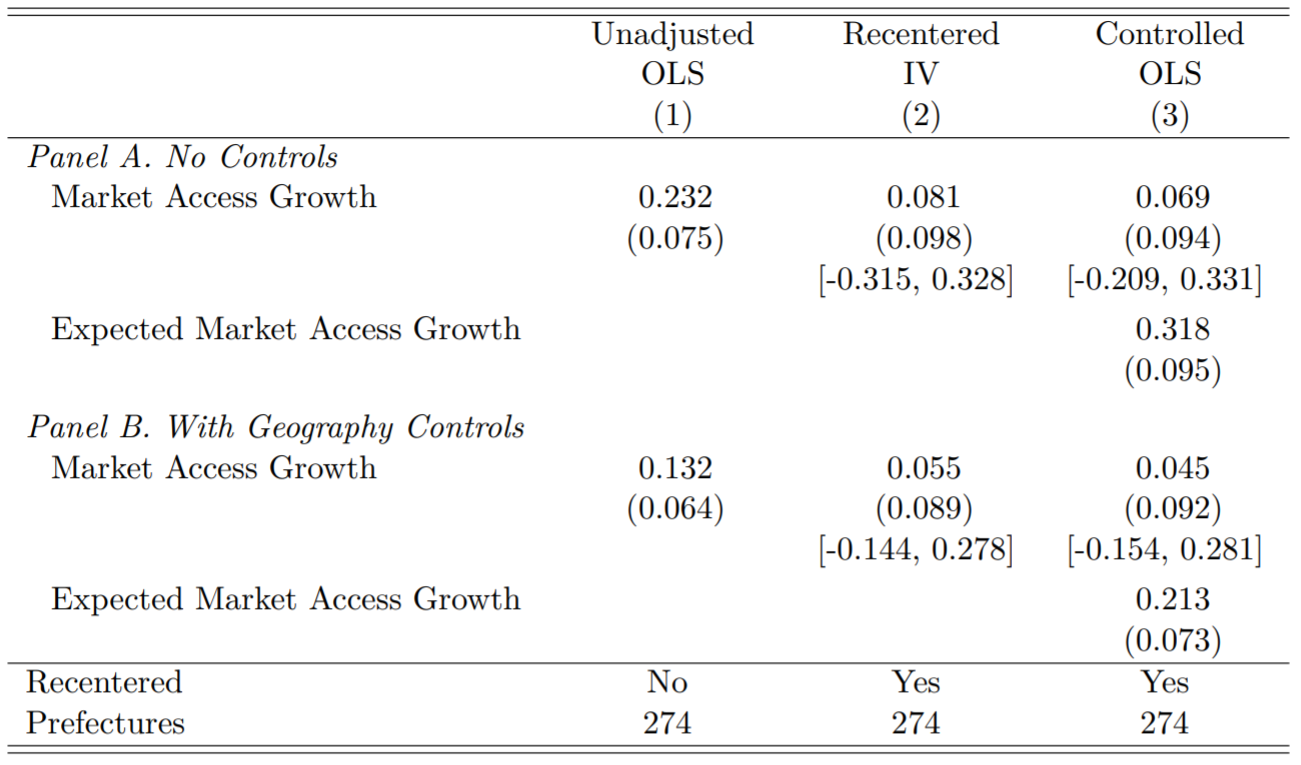
\includegraphics[width=0.9\textwidth]{figures/hsr_tab.png}
\end{center}

Large effect for naive OLS goes away with recentering/controlling \smallskip
\begin{itemize}
\item Once adjusting for $\mu_i$, auxilliary controls don't matter ($\implies$ balance)
\end{itemize}

\end{frame}

\begin{frame}{Inference Can Be Tricky with Formulas}

\begin{itemize}
\item Common exposure to the exogenous shocks $g$ make $z_i=f_i(g,s)$ correlated across $i$, potentially in complicated ways\smallskip
\begin{itemize}
\item E.g. for shift-share $z_i=\sum_k s_{ik}g_k$, if unit $i$ and $j$ are far apart in space but close in terms of $(s_{ik})_{k=1}^K$ and $(s_{jk})_{k=1}^K$ then $Cov(z_i,z_j)>0$ \smallskip\pause{}
\item Following our Day 2 discussion, this suggests we should cluster $i$ and $j$ together.\pause{} But how do we do this? Shares are not ``groups''
\end{itemize}\bigskip\pause{}
\item For SSIV, Borusyak et al. (2022) show there is an equivalent shock-level IV that yields ``exposure-robust'' standard errors with ``, r''\smallskip
\begin{itemize}
\item Intuitively: address ``clustering'' by running the IV at the level of identifying variation. Stata/R package: \emph{ssaggregate}
\end{itemize}\bigskip\pause{}
\item For other $f_i(\cdot)$, Borusyak and Hull '23 propose randomization inference\smallskip
\begin{itemize}
\item Use the counterfactual $g$ to simulate the distribution of test statistics under the null and check if the actual test is in the tails
\end{itemize}
\end{itemize}
\end{frame}


\begin{frame}{Outline}

\textcolor{red!75!green!50!blue!25!gray}{1. Formula Treatments/Instruments}$\checkmark$
\vspace{0.8cm}

2. Structural Models

\end{frame}

\begin{frame}{Models as Extrapolators}
\begin{itemize}
\item I've focused on \emph{linear} regression/IV procedures, showing that they can estimate certain convex averages of heterogeneous effects given design\smallskip\pause
\begin{itemize}
\item But such effects needn't coincide w/policy-relevant param's (e.g. ATE)
\end{itemize}\bigskip\pause{}
\item Intuitively, we can try to bridge this gap by putting additional structure on (otherwise non-parametric) potential outcomes\smallskip\pause{}
\begin{itemize}
\item In fact, we've already seen this: our Day-1 constant-effect model of $y_i=\beta x_i+\varepsilon_i$ can be understood as extrapolating simply across all $i$\smallskip\pause{}
\item Other (nonlinear) procedures can sometimes be seen as imposing different extrapolations to the same underlying (design-based) variation
\end{itemize}
\end{itemize}
\end{frame}

\begin{frame}{Simple Example: OLS vs. Probit}
\begin{itemize}
\item Suppose individuals with baseline covariate $w_i=1$ are randomized into a treatment $x_i\in\{0,1\}$. Those with $w_i=0$ are all untreated\smallskip\pause{}
\begin{itemize}
\item Q: What do we get from regressing $y_i$ on $x_i$ controlling for $w_i$?\smallskip\pause{}
\item A: The CATE $E[y_i(1)-y_i(0)\mid w_i=1]$, since $Var(x_i\mid w_i=0)=0$\smallskip\pause{}
\item Taking the linear regression/model for $E[y_i\mid x_i,w_i]$ seriously, this is also our estimate of the (otherwise unidentified) $E[y_i(1)-y_i(0)\mid w_i=0]$
\end{itemize}\bigskip\pause{}
\item Suppose $y_i$ is binary and we instead run a Probit on $x_i$ and $w_i$\smallskip
\begin{itemize}
\item Taking it seriously, Probit structures potential outcomes:
\begin{align*}
 y_i=& \mathbf{1}[\alpha+\beta x_i+\gamma w_i\ge\varepsilon_i],\hspace{0.3cm} \varepsilon_i\mid x_i,w_i\sim N(0,1) \\
\pause{} \implies &  y_i(0)=\mathbf{1}[\alpha+\gamma w_i\ge \varepsilon_i],\hspace{0.2cm}y_i(1)=\mathbf{1}[\alpha+\beta + \gamma w_i\ge \varepsilon_i]
\end{align*}\pause{}\vspace{-0.2cm}
\item In particular, $E[y_i(1)-y_i(0)\mid w_i=1]=\Phi(\alpha+\beta+\gamma)-\Phi(\alpha+\gamma)$ (will match OLS) but $E[y_i(1)-y_i(0)\mid w_i=0]=\Phi(\alpha+\beta)-\Phi(\alpha)$\smallskip\pause{}
\item Different extrapolation of missing CATE: a feature or a bug?
\end{itemize}
\end{itemize}
\end{frame}

\begin{frame}{ExtrapoLATEing}

\begin{itemize}
\item Consider the simplest design-based IV story: binary $x_i$, binary $z_i$, no controls. IV identifies LATE:
\begin{align*}
\beta^{IV} = E[y_i(1)-y_i(0)\mid x_i(1)>x_i(0)]
\end{align*}
where $x_i(z)$ denotes potential treatment when $z_i=z$\smallskip
\begin{itemize}
\item Avg. treatment effect among compliers (those with $x_i(1)=1, x_i(0)=0$)
\end{itemize}\bigskip\pause{}
\item Without restrictions on $(y_i(1),y_i(0),x_i(1),x_i(0))$, can't say anything more: IV only reveals effects among $i$ whose $x_i$ is shifted by $z_i$\smallskip\pause{}
\begin{itemize}
\item Actually not quite true: can identify avg. $y_i(1)$ of always-takers (w/ $x_i(1)=x_i(0)=1$), avg. $y_i(0)$ of never-takers (w/ $x_i(1)=x_i(0)=0$), as well as avg. $y_i(1)$ \& $y_i(0)$ separately for compliers 
\smallskip
\item By adding a (semi-)parametric model of selection, we can extrapolate these objects to identify other parameters, e.g., ATE $E[y_i(1)-y_i(0)]$
\end{itemize}
\end{itemize}
\end{frame}

\begin{frame}{Adding Structure to IV}

Suppose we have a $z_i$ which is as-good-as-randomly assigned + excludable\smallskip
\begin{itemize}
\item Assume a distribution for $(y_i(1),y_i(0),\nu_i)$ where $x_i=\mathbf{1}[\mu+\pi z_i>\nu_i]$\smallskip\pause{}
\item Then we have parametric models for
\begin{align*}
E[y_i\mid x_i=1,z_i=z]&=E[y_i(1)\mid \mu+\pi z>\nu_i]\equiv f_1(z;\theta)\\
E[y_i\mid x_i=0,z_i=z]&=E[y_i(0)\mid \mu+\pi z<\nu_i]\equiv f_0(z;\theta)
\end{align*}
as well as ``first stage'' models for $Pr(x_i=1\mid z_i=z)=g(z;\theta)$ \pause{}\medskip
\item With enough variation in $z_i$, the parameter vector $\theta$ (and thus ATE) can be identified from these moment restrictions 
\end{itemize}\bigskip\pause{}

Key point: the model allows us to extrapolate ``local'' IV variation to estimate more ``policy relevant'' parameters\smallskip
\begin{itemize}
\item When $z_i$ has limited support, the model is doing more ``work''\smallskip
\item With full support, we have ``identification at infinity'' (w/o a model)
\end{itemize}

\end{frame}

\begin{frame}{Linking Back to LATE}

\vspace{0.2cm}
Kline and Walters (2019) formalize this extrapolation logic in the familiar Imbens and Angrist (1994) setup\smallskip
\begin{itemize}
\item Key result: in simple binary $z_i$ / no controls setup, control function estimates of LATE are numerically identical to linear IV\smallskip\pause{}
\item ``Differences between structural and IV estimates therefore stem in canonical cases entirely from disagreements about the target parameter rather than from functional form assumptions'' (p. 678)\smallskip\pause{}
\item Functional form instead shapes the extrapolation to other parameters (as in our earlier probit example!)
\end{itemize}\bigskip\pause{}

All of this can be extended to conditional as-good-as-random assignment 
\begin{itemize}
\item Design knowledge gives you reduced-form estimands; then plug these into a model to get more!
\end{itemize}

\end{frame}

\begin{frame}{Heckit Extrapolation of IV Moments}

\begin{center}
	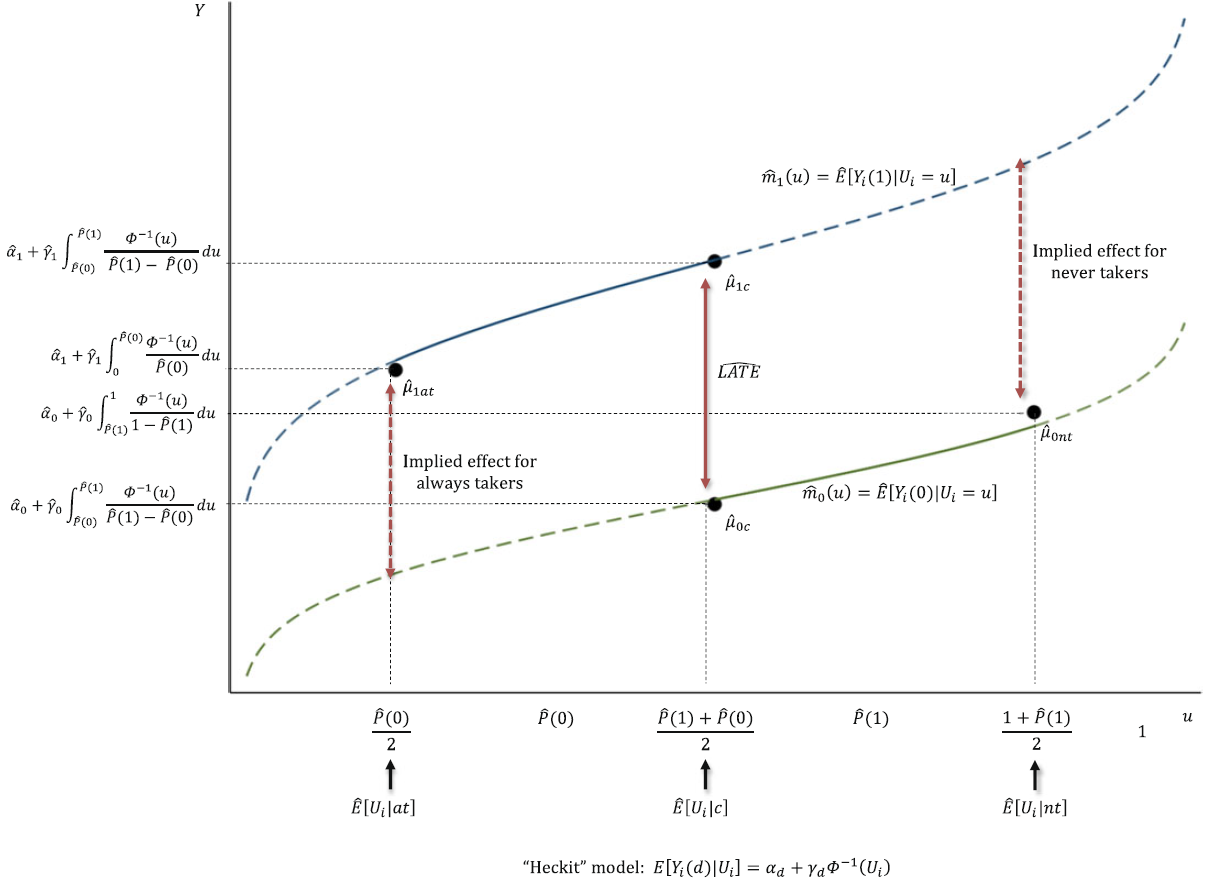
\includegraphics[width=0.95\textwidth]{figures/kw_heckit.png}
\end{center}
\end{frame}

\begin{frame}{Summing Up}
\begin{itemize}
\item You can do a lot with a solid design-based identification strategy\smallskip
\begin{itemize}
\item Give a clear \emph{ex ante} rationalization for controls in a linear regression/IV\smallskip
\item Have confidence in the level of standard error clustering\smallskip
\item Avoid concerns over ``negative weights'' / explore alternative weightings\smallskip
\item Understand what economic models buy you for identification
\end{itemize}\bigskip\pause{}
\item Of course, design is not the only way to go: outcome modeling (e.g. DiD) may be a good alternative, especially w/o good shock variation\smallskip
\begin{itemize}
\item But some of the above issues can get murkier -- just be clear on what you're assuming!
\end{itemize}\bigskip\pause{}

\begin{center}
\textbf{Thanks for a Great Class!}
\end{center}
\end{itemize}

\end{frame}

\end{document}
}
